\documentclass[tikz,border=2pt]{standalone}
\usepackage{amsmath}
\usetikzlibrary{arrows.meta}
\begin{document}
% A = [[1,-2],[1,3]]: eigenvalues 2 +- i, mirror images in the real axis with modulus
% rho = sqrt5 and angles +- theta, theta = arctan(1/2) (left). With p = u + iw, u = (-1,1)^T,
% w = (1,0)^T, the matrix keeps the real plane span{u,w}: Au = (-3,2)^T = 2u - w (right).
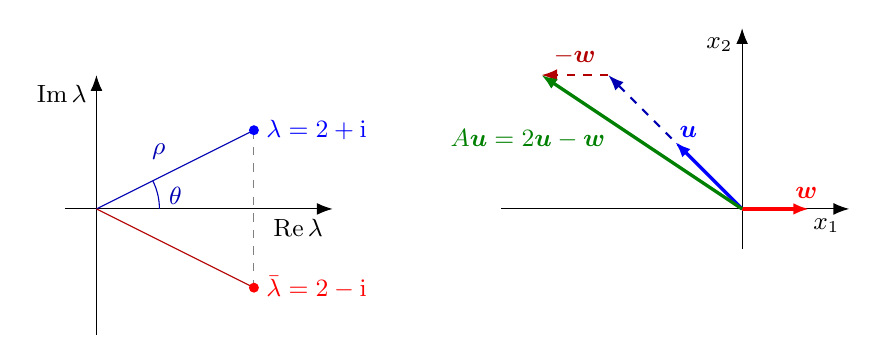
\begin{tikzpicture}[font=\small, >={Latex[length=2mm]}]
  % left: complex plane
  \begin{scope}[x=1.0cm, y=1.0cm]
    \draw[->] (-0.4,0) -- (3.0,0) node[below left] {$\operatorname{Re}\lambda$};
    \draw[->] (0,-1.6) -- (0,1.7) node[below left] {$\operatorname{Im}\lambda$};
    \draw[gray, thin, dashed] (2,1) -- (2,-1);
    \draw[blue!70!black, thin] (0,0) -- (2,1);
    \draw[red!70!black, thin] (0,0) -- (2,-1);
    \draw[blue!70!black, thin] (0.8,0) arc[start angle=0, end angle=26.57, radius=0.8];
    \node[blue!70!black, anchor=west] at (0.8,0.17) {$\theta$};
    \node[blue!70!black, anchor=south east] at (1.0,0.5) {$\rho$};
    \fill[blue] (2,1) circle (1.8pt) node[right, xshift=1pt] {$\lambda=2+\mathrm{i}$};
    \fill[red] (2,-1) circle (1.8pt) node[right, xshift=1pt] {$\bar\lambda=2-\mathrm{i}$};
  \end{scope}
  % right: real plane span{u,w}
  \begin{scope}[xshift=8.2cm, x=0.85cm, y=0.85cm]
    \draw[->] (-3.6,0) -- (1.6,0) node[below left] {$x_1$};
    \draw[->] (0,-0.6) -- (0,2.7) node[below left] {$x_2$};
    \draw[->, blue!70!black, thick, dashed] (0,0) -- (-2,2);
    \draw[->, red!70!black, thick, dashed] (-2,2) -- (-3,2);
    \node[red!70!black, anchor=south] at (-2.5,2) {$-\boldsymbol{w}$};
    \draw[->, blue, very thick] (0,0) -- (-1,1) node[above right, inner sep=1pt] {$\boldsymbol{u}$};
    \draw[->, red, very thick] (0,0) -- (1,0) node[above, xshift=-1pt] {$\boldsymbol{w}$};
    \draw[->, green!50!black, very thick] (0,0) -- (-3,2);
    \node[green!50!black, anchor=east] at (-1.9,1.05) {$A\boldsymbol{u}=2\boldsymbol{u}-\boldsymbol{w}$};
  \end{scope}
\end{tikzpicture}
\end{document}
